\documentclass[a4paper,11pt,pdf]{pacmanreport}

\usepackage{helvet}
\usepackage{graphicx}

%%=== Aditional packages
%\usepackage{hyperref} % references
\usepackage{amssymb}
\usepackage{tikz}

\usetikzlibrary{shapes,arrows}
\usepackage{mathtools}
\usepackage{float}
\usepackage{subcaption}

\usepackage[bookmarks=true,hyperfootnotes=true]{hyperref}
\hypersetup{
			colorlinks=true,
			linkcolor=blue,
			anchorcolor=blue,
			citecolor=blue,
			urlcolor=blue,
            filecolor=blue,
			pdftitle={Milestone 4.2}
}

%%=====================


\graphicspath{{images/}{../shared_images/}{images/plots/}}

%% ================================
%% PROJECT INFO 

\project{}
\projectid{FP7-IST-60918}
\projectstart{1 March 2013}
\duration{36}

%% ================================
%% MILESTONE INFO 

\title{Reactive haptic exploration control strategies ready for integration with planning}
\deliverableid{Milestone 4.2}
\author{M. Bonilla, C. Rosales, M. Gabiccini}
\address{Centro di Ricerca ``E. Piaggio'', Universit\`{a} di Pisa}
\email{manuel.bonilla@centropiaggio.unipi.t}
\headertitle{Exploration strategies}
\headerauthor{M. Bonilla, C. Rosales, M. Gabiccini}
\duedate{2015-02-28}
\submissiondate{2014-02-28}
\leadpartner{Universit\`{a} di Pisa}
\revision{draft}
\disseminationlevel{PU}

%% UNCOMMENT: to get the logo; if you've copied this file to a directory yearX/wpY/ then this should work
\reportlogo{pacmanlogo.png}

%!TEX root = MS42.te
%% ======= Defining tikz style
\tikzstyle{block} = [draw, fill=blue!5, rectangle, 
    minimum height=3em, minimum width=6em]
\tikzstyle{block_small} = [draw, fill=blue!5, rectangle, 
    minimum height=3em, minimum width=3em]
\tikzstyle{sum} = [draw, fill=blue!5, circle]
\tikzstyle{intersection} = [fill,circle,minimum size=3pt,inner sep=0pt]
\tikzstyle{input} = [coordinate]
\tikzstyle{output} = [coordinate]
%%==============


\begin{document}

\maketitle

\begin{abstract}
\noindent This milestone detail the work performed to integrate planning and execution phases involving object exploration and grasping, and potentially gaze control. 
\end{abstract}


\vspace{.2em}
\hrule

\vspace{.2em}
\footnotesize

\tableofcontents

\normalsize

\newpage

\section{Milestone Summary and Context}

This milestone describes the work performed to integrate planning and execution phases concerning object exploration and grasping using a bimanual robot.

%The main contributions are 1) the technical implementation of hardware interfaces to command the KUKA LWR arm using ROS and 2)  the implementation of different classical controllers to move the robot using torque references.

%The first contribution is useful to command the robot using torque commands easier that using the actual KUKA FRI interface. The second helps to execute trajectories coming from planning phase, and to move the robot to desired references under different situations such as dynamic model uncertainty and different redundancy resolution at kinematic and dynamic levels. 

The platform presented in this milestone should be of great importance in the implementation, testing and validation of the development algorithms within the PaCMan project.


%In recent years, there has been growing interest in the development of a standardized framework for robotic implementations, where the robots interdisciplinary code and software could be easy to write and accessible to everyone. This is the philosophy of the \textit{Robot Operating System} (\textbf{ROS}), a flexible framework which provides all the instruments to develop and build robust and robot-independent applications, allowing researchers from different fields of robotics to share each others works with the great result of spreading the know-how.

Since ROS is the software framework used in PaCMan we developed a hardware interface for the robots used in the experimental platforms. However, this interface is just useful to command the robot using torque references. There are different strategies to generate the torque references to move a robot manipulator, they are designed for different situation for example under uncertainty, which main problem faced in PaCMan Project, in this case in the robot dynamics. Other strategies to deal with multi-goal references at kinematic and dynamic level were also implemented.

% What was the milestone that you are examining? What were the criteria for achieving it? What role does achievement of the milestone play in the whole project? How will its achievement as presented in this report contribute to the PaCMan scenarios and prototypes? 

% \subsection{Project Goals}

% The aim of this milestone report is focused on the development of a ROS-enabled software environment for controlling the manipulator KUKA LWR IV, used in the PaCMan platforms. 

After a first phase of studying and analyzing some of the novel approaches for robot control, the default control strategies provided by the manufacturer has been extended, implementing a new set of controllers.
The development of the controllers, including tuning and debugging, has been realized with the support of \textit{Gazebo}, a high performance realistic simulator which, interacting with ROS, gives the opportunity to test the efficiency of user-implemented control algorithms. 

%Finally, the last phase consisted in pursuing experiments to test the implemented control strategies on the physical robot, arising a variety of practical issues which don't come out in simulation, that are explained in detail in this document.


The software here exposed can be found in the project website~\cite{PACMAN_software}.

% \newpage

\section{Report on Milestone Achievement}

% How have the tasks been addressed? To what extent have the intended objectives been achieved? Why, how -- or why not? In particular what concrete acceptance tests, or experimental results show that the milestone has been achieved.


% \section{Annexes}

% Here you should briefly describe the papers attached that provide evidence for achievement of the milestone. Mention titles, authors, publication info; abstract; and a one-liner relating the publication back to the discussion on actual work performed. 


%!TEX root = MS42.te
%% ======= Defining tikz style
\tikzstyle{block} = [draw, fill=blue!5, rectangle, 
    minimum height=3em, minimum width=6em]
\tikzstyle{block_small} = [draw, fill=blue!5, rectangle, 
    minimum height=3em, minimum width=3em]
\tikzstyle{sum} = [draw, fill=blue!5, circle]
\tikzstyle{intersection} = [fill,circle,minimum size=3pt,inner sep=0pt]
\tikzstyle{input} = [coordinate]
\tikzstyle{output} = [coordinate]
%%==============
\subsection{Software: Vito, the UNIPI robot, package}
\label{sec:vito}

Vito, the UNIPI robot, is the younger brother of Eddie and Boris, the UIBK and UoB robots, respectively. It is a bi-manual robot with a high quality head. The difference with the other two robots is that Vito uses two Pisa/IIT SoftHands as end-effectors as the default setup. However, its modularity allows him to exchange tools such as a DLR hand, an intrinsic tactile sensors like the one used in DR 3.1, or as an object scanner when using an RGB-D camera and a turntable. Fig.~\ref{fig:vito_gazebo} shows Vito uploaded in the Gazebo environment. The package is accessible through the project website~\cite{PACMAN_software}.

\begin{figure}[h]
\centering
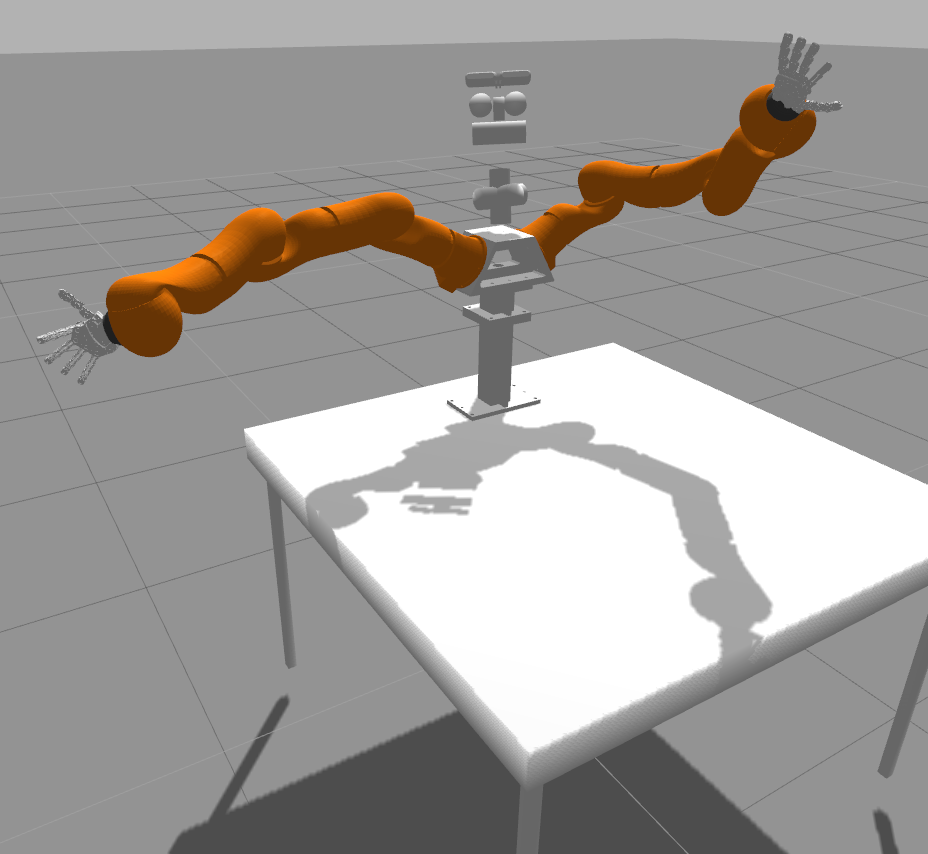
\includegraphics[width=0.7\textwidth]{vito_gazebo.png}
\caption{Vito, the UNIPI robot, in the ROS/Gazebo simulation.}
\label{fig:vito_gazebo}
\end{figure}

\subsubsection{Models and modularity}

All modules, namely the KUKA LWR arm (Sec.~\ref{sec:kuka}, the Pisa/IIT SoftHand (Sec.~\ref{sec:softhand}) and KIT Head (Sec.~\ref{sec:kithead}), were developed in such manner that they can be instantiated to create more complex robots like Vito in a very easy and moddular way. In Fig~\ref{fig:vito}, or by clicking \href{https://github.com/CentroEPiaggio/vito_robot/blob/master/vito_description/robot/vito.urdf.xacro}{here}, you can see the actual complete specification of the Vito model. On the top, you see the inclusion of the models, some of them are specific to the robot, such as the torso, table, and couplers, and others are imported such as the arm, hand and head.

\begin{figure}
\tiny
\begin{verbatim}
<?xml version="1.0"?>
<robot xmlns:xacro="http://www.ros.org/wiki/xacro" 
       name="vito">
       
  <!-- MODELS -->
  <xacro:include filename="$(find vito_description)/model/torso.urdf.xacro"/>
  <xacro:include filename="$(find vito_description)/model/table.urdf.xacro"/>
  <xacro:include filename="$(find vito_description)/model/materials.urdf"/>
  <xacro:include filename="$(find vito_description)/model/clamp.urdf.xacro"/>
  <xacro:include filename="$(find vito_description)/model/softhand_base.urdf.xacro"/>
  <xacro:include filename="$(find lwr_description)/model/kuka_lwr.urdf.xacro"/>
  <xacro:include filename="$(find soft_hand_description)/model/soft_hand.urdf.xacro"/>
  <xacro:include filename="$(find kit_head_description)/model/kit_head.urdf.xacro"/>
    
  <link name="world" />
  
  <!-- TABLE -->
  <xacro:model_table name="table" 
                    parent="world"
                    length="1.45"
                    width="1.45"
                    height="0.9"
                    plate_thickness="0.1">
    <origin xyz="-1.22 0.75 0" rpy="0 0 0"/>
  </xacro:model_table>

  <!-- TORSO -->
  <xacro:model_torso name="torso" parent="world">
    <origin xyz="0 0 0"/>
  </xacro:model_torso>
  
  <!-- LEFT ARM -->
  <xacro:kuka_lwr name="left_arm" parent="world">
    <origin xyz="0.0 -0.108585 0.475" 
      rpy="${M_PI*40.8933907/180} ${M_PI*48.5903708/180} ${M_PI*-40.8933907/180}"/>
  </xacro:kuka_lwr>

  <!-- LEFT COUPLERS -->
  <xacro:clamp name="left_clamp" parent="left_arm_7_link">
    <origin xyz="0 0 0.01" rpy="0 0 0"/>
  </xacro:clamp>

  <xacro:softhand_base name="left_base" parent="left_clamp" left="true">
    <origin xyz="0 0 0.004" rpy="0 0 0"/>
  </xacro:softhand_base>

  <!-- LEFT SOFTHAND -->
  <xacro:soft_hand parent="left_base" name="left_hand" left="true" withAdaptiveTransmission="true" useMimicTag="false">
    <origin xyz="0 0 0.0535" rpy="0 0 0"/>
  </xacro:soft_hand>

  <!-- RIGHT ARM -->
  <xacro:kuka_lwr name="right_arm" parent="world">
    <origin xyz="0.0 0.108585 0.475" 
      rpy="${M_PI*-40.8933907/180} ${M_PI*48.5903708/180} ${M_PI*40.8933907/180}"/>
  </xacro:kuka_lwr>

  <!-- RIGHT COUPLERS -->
  <xacro:clamp name="right_clamp" parent="right_arm_7_link">
    <origin xyz="0 0 0.01" rpy="0 0 0"/>
  </xacro:clamp>

  <xacro:softhand_base name="right_base" parent="right_clamp" left="false">
    <origin xyz="0 0 0.004" rpy="0 0 0"/>
  </xacro:softhand_base>

  <!-- RIGHT SOFTHAND -->
  <xacro:soft_hand parent="right_base" name="right_hand" left="false" withAdaptiveTransmission="true" useMimicTag="false">
    <origin xyz="0 0 0.0535" rpy="0 0 0"/>
  </xacro:soft_hand>

  <!-- HEAD -->
  <xacro:kit_head name="head" parent="world">
    <origin xyz="0.0 0.0 ${0.55 + 0.1}" rpy="0.0 0.0 3.141592"/>
  </xacro:kit_head>

</robot>
\end{verbatim}
\caption{Vito definition using the available models as components.}
\label{fig:vito}
\end{figure}


\subsubsection{Real/Simulation planning and control framework}

The planning framework is heavily based on the MoveIt! package, since motion planning is not within the goals of the project. It is worth to mention that Section ``High-Level Planning for Dual Arm Goal-Oriented Task'' in DR 4.2 interfaces with the core planning functions of the package to generate and use the transition graph.

For the control framework, each module implements an interface to the real or the simulated hardware, looking for maximum similarities between the two scenarios to have a switch between reality and simulation as effortless as possible. Both hardware interfaces expose the joints as resources that can be controlled using effort, position, or even velocity commands. This depends on the available hardware. Moreover, controllers that are compatible with the resources exposed by the hardware interface can be used indistinctly. All controllers are gathered in a configuration file that defines its functional parameters, such as the proportional, derivative and integral gains in a PID controller. Such controllers are listed as the way a group of joints can be moved in a regulated way to execute trajectories, perform exploration, or move to any desired position in the workspace. Given the fact that the main PaCMan contribution is not on trajectory planning, we decided to use the MoveIt! library to tackle this aspect.

The plan-to-action framework can be summarized in Fig.~\ref{fig:framework}. The link between the two figures is the controllers, in the sense that they must understand the planning output, typically joint trajectories, and the commanded values must be compatible with the hardware resource types, typically position and effort commands.

\begin{figure}
\centering
\begin{subfigure}[t]{0.58\textwidth}
\centerline{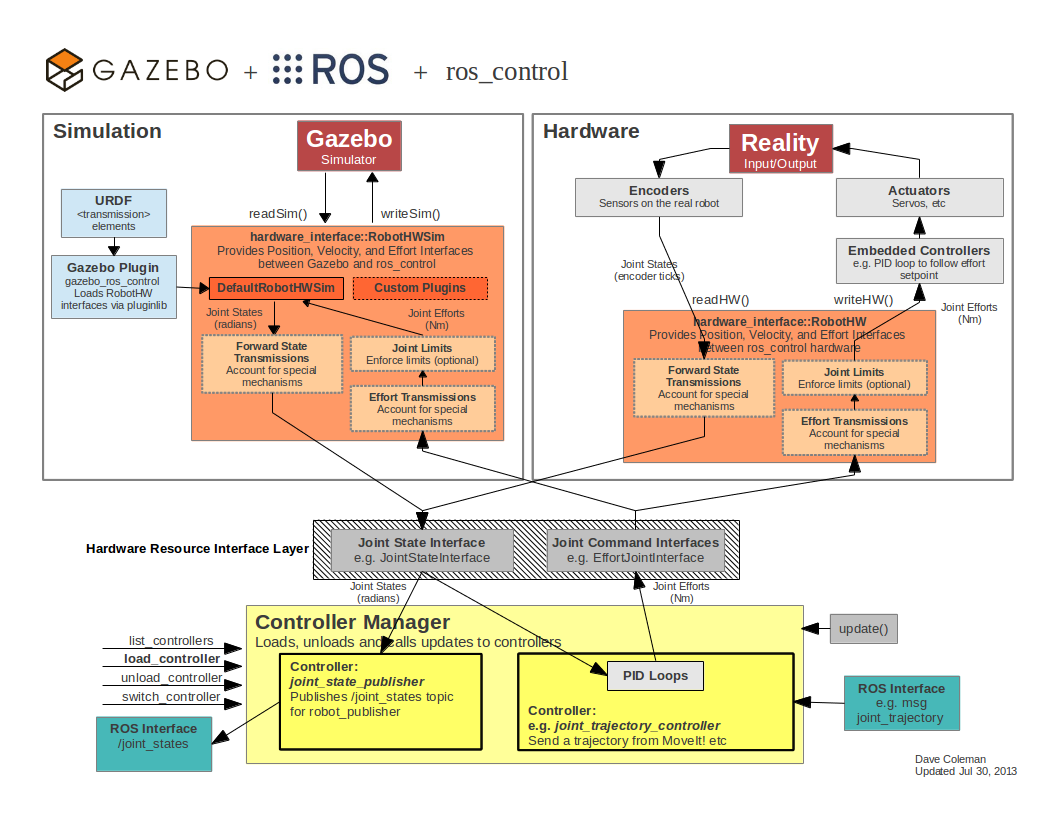
\includegraphics[width=\textwidth]{ros+gazebo.png}}
\caption{ROS/Gazebo framework.}
\label{fig:rosgazebointeraction}
\end{subfigure}
\begin{subfigure}[t]{0.4\textwidth}
\centerline{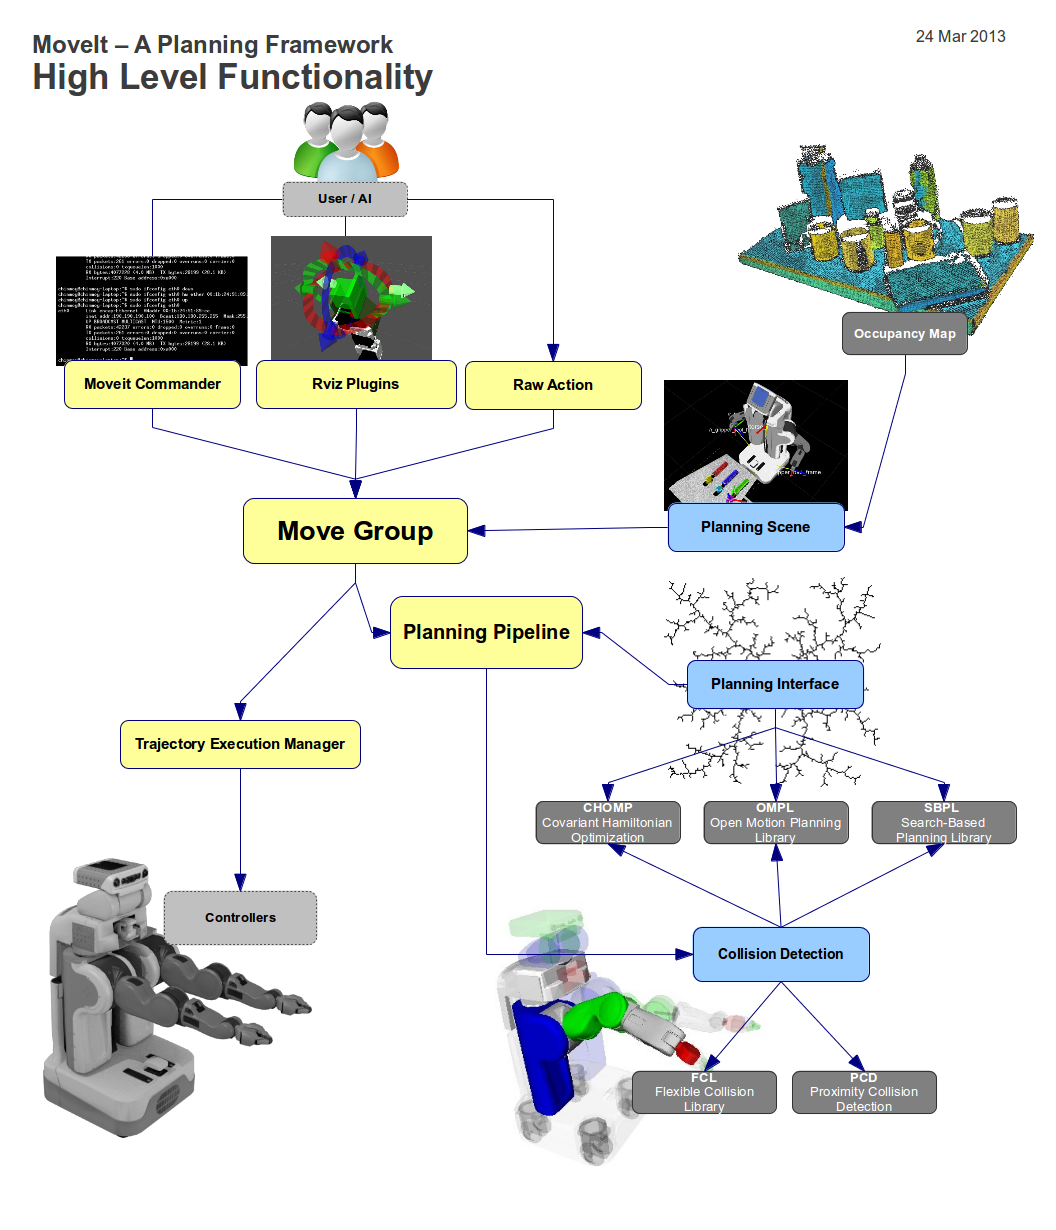
\includegraphics[width=\textwidth]{moveit_highlevel.png}}
\caption{MoveIt! framework.}
\label{fig:planning}
\end{subfigure}
\caption{Real/Simulation planning and control framework}
\label{fig:framework}
\end{figure}

Particularly, the arm~(see Sec.~\ref{sec:kuka}) works with both effort and position using the same hardware interface in both real and simulation, and the hand (see Sec.~\ref{sec:softhand}) and head~(see Sec.~\ref{sec:kithead}) offer only position controlled motors. Next, we describe more details on the hardware interface of each module. In the case of the arm, special attention is given to the implementation of additional controllers that make the most of the arm capabilities for the required tasks within the project. In the case of the hand, special attention is given to the implementation of the adaptive synergy transmission to replicate in simulation the adaptivity the hand has in reality.
%With this in mind, the planning and execution phase  at a robust object exploration and grasping.
%!TEX root = MS42.tex
\section{The Robot}\label{sec:therobot}
\subsection{KUKA LWR IV}

The robot used for the project experiments, the \textit{KUKA Lightweight Robot IV} \cite{webkuka}, is a 7-axis industrial manipulator which finds a wide employment in the field of the robotics research due to its flexibility and modularity, including a payload capacity of 7 Kg. In addition, the seventh axis makes the robot redundant, which mean that, for a given position and orientation of the end effector, there exist multiple configurations in the joints space. Each joint is equipped with a position and a torque sensor, allowing the robot to be operated with position, velocity and torque control. 

\begin{figure}[h]
\centering
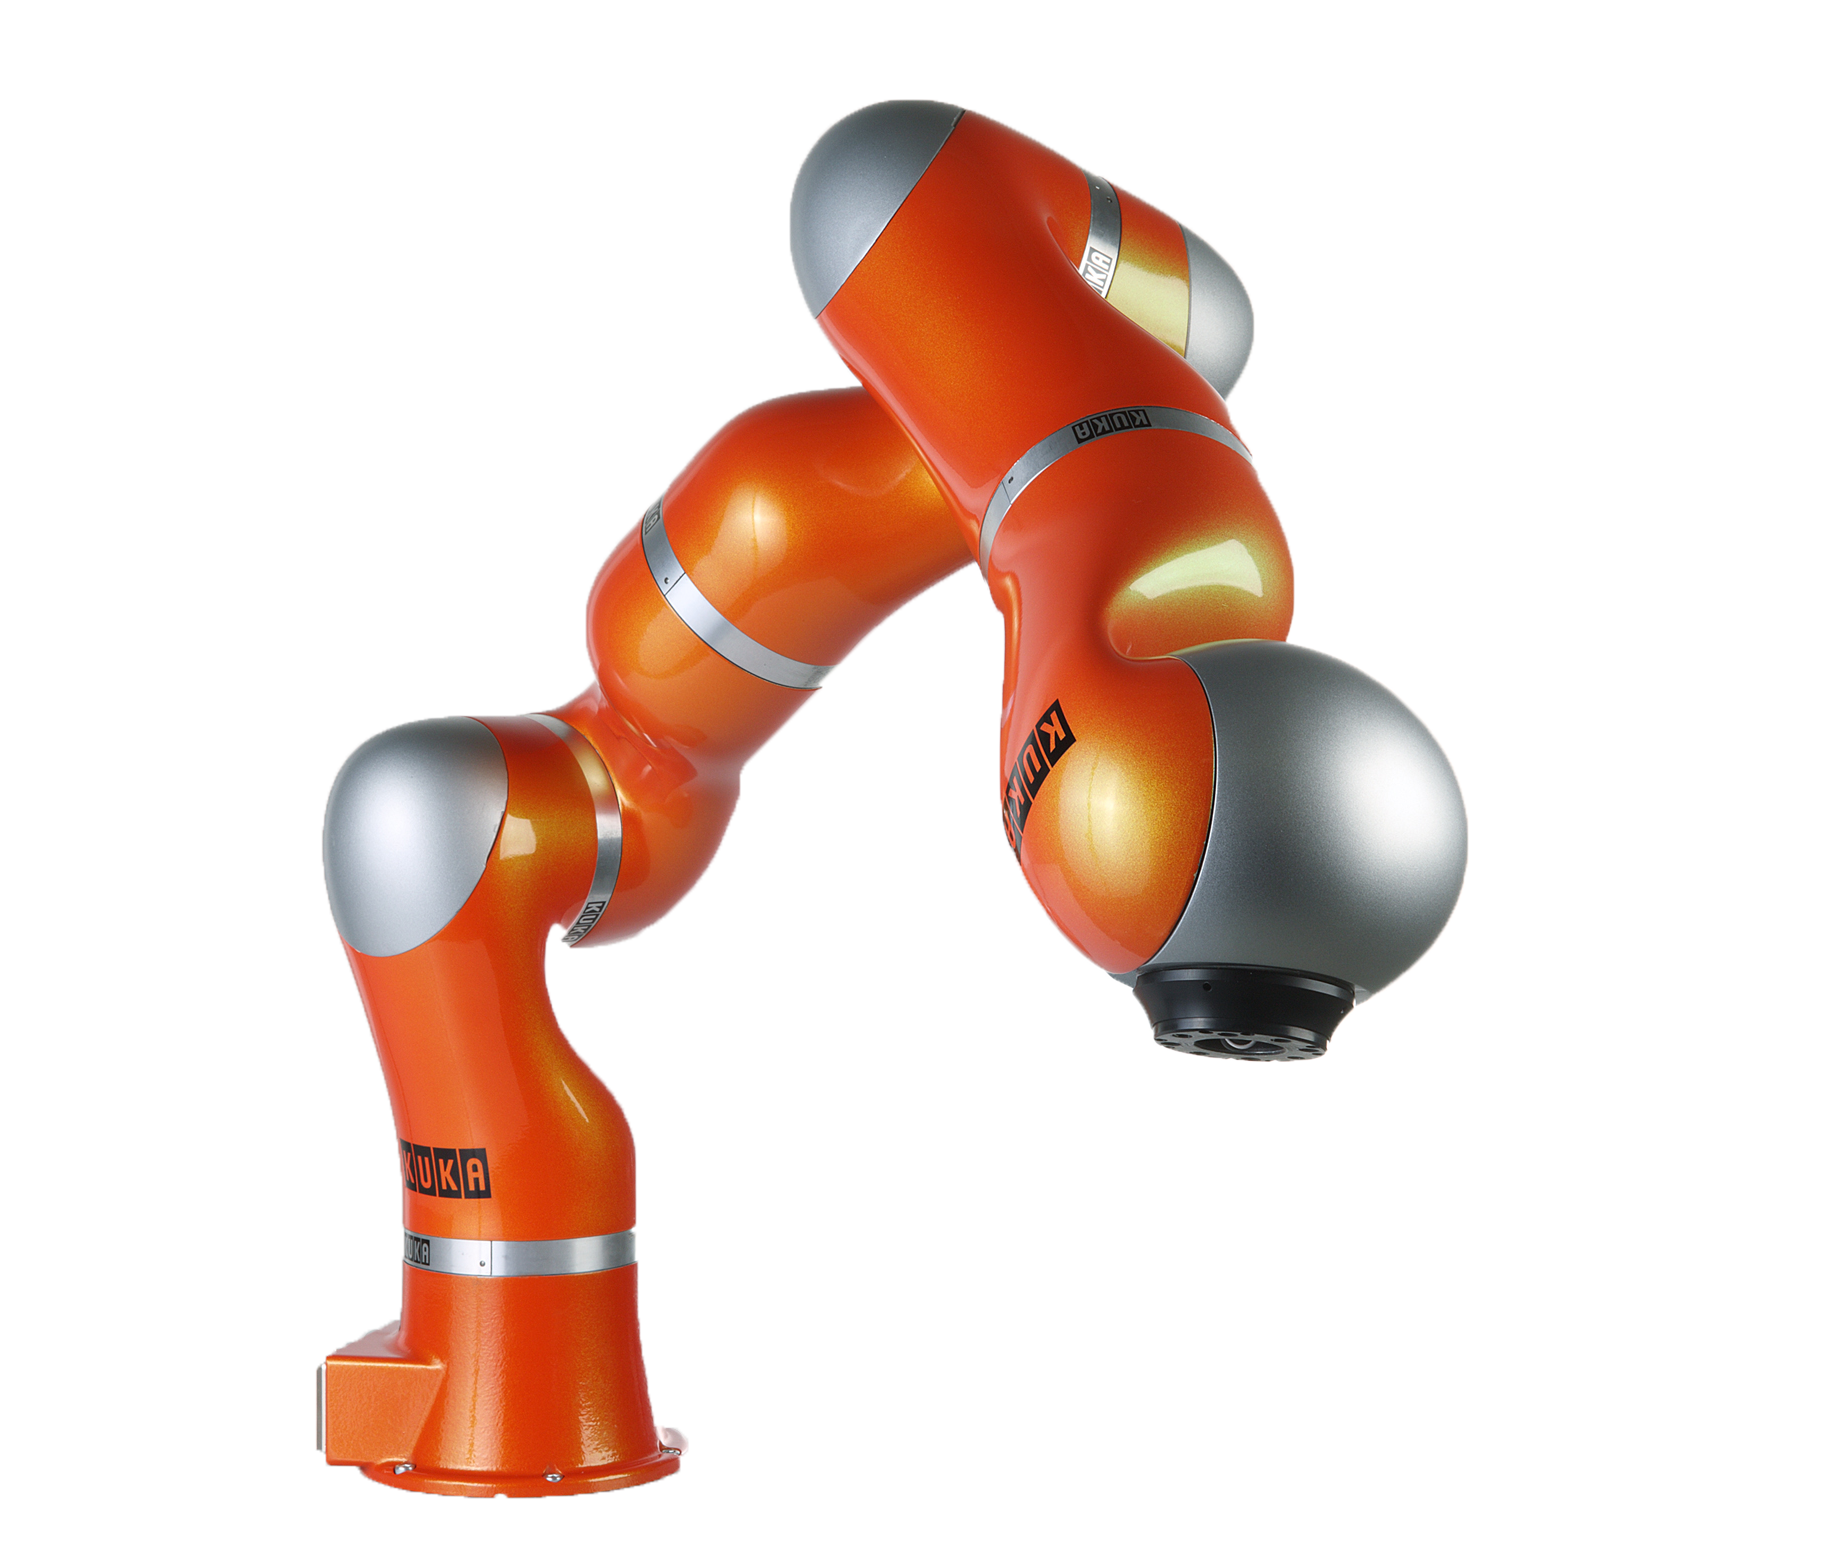
\includegraphics[scale=0.7]{kuka}
\caption{KUKA Lightweight Robot IV arm}
\end{figure}

The communication between the robot and an external computer is handled by the \textit{Fast Research Interface} (FRI), a real-time proprietary software interface able to read and write system variables of the robot and execute user-programs.

\subsection{Built-in Control Strategies}
The robot provides three different control strategies as default setting, which are described below.
\subsubsection*{Position Controller}
The position controller takes as command the desired joints set-point position, ensuring regulation through the use of an internal \textit{PID}. 

\subsubsection*{Cartesian Stiffness Controller}
The Cartesian stiffness controller is characterized by the following control law:
\begin{equation}
\tau_{cmd} = J^T(k_c(x_{FRI} - x_{msr}) + F_{FRI}) + D(d_c) + f_{dynamics}(q,\dot{q},\ddot{q})
\label{eq:cartesianstiffnesscontroller}
\end{equation}

where:
\begin{itemize}
\item $x_{FRI}$: cartesian commanded set-point position;
\item $k_c$: cartesian stiffness;
\item $D(d_c)$: damping term;
\item $f_{dynamics}(q,\dot{q},\ddot{q})$: the dynamic model;
\item $F_{FRI}$: the cartesian force.
\end{itemize}

\subsubsection*{Axis-specific Stiffness Controller}
The axis-specific stiffness controller is similar to the cartesian stiffness controller, but it takes commands in joints space:
\begin{equation}
\tau_{cmd} = (k_j(q_{FRI} - q_{msr}) + \tau_{FRI}) + D(d_j) + f_{dynamics}(q,\dot{q},\ddot{q})
\label{eq:axisspecificstiffnesscontroller}
\end{equation}

\newpage
\subsection{Pisa/IIT SoftHand}
\label{sec:softhand}

The Pisa/IIT SoftHand is a 5-finger hand that introduces an implementation of the adaptive synergy transmission~\cite{Catalano2014Adaptive}. Fig~\ref{fig:soft_hand}.

\begin{figure}[b]
\centering
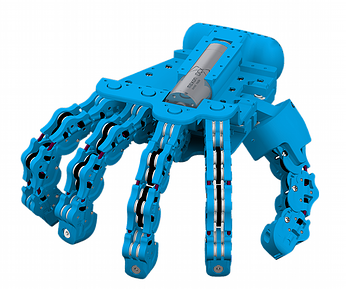
\includegraphics[width=0.4\textwidth]{soft_hand.png}
\caption{The Pisa/IIT SoftHand, 1 motor and 19 dof.}
\label{fig:soft_hand}
\end{figure}

\subsubsection{Hardware interface}

The real hardware interface is implemented using the API provided by qbrobotics$^{\copyright}$~\cite{qbrobotics_software}, using position commands. 

The simulated hardware interface is special. 

The interface is loaded into Gazebo as a plug-in that has access to the simulation, useful to read the full hand state as well as contacts, and receives commands from the controller in position. To simulate the SoftHand behavior the four elements described below are used within the interface implementation.

\paragraph{Joint description} The knuckle joint for all fingers is a regular revolute joint, so they are specified as such using common URDF tags~\ref{webros}. The inter-phalangeal joints, however, are based compliant rolling-contact joints, which are not among the library of joint types in any of the simulation environments available today, as far as the authors know. Thus, it requires a special treatment to emulate the kinematic motion resulting from rolling. To this end, each inter-phalangeal joint is the combination of two revolute joints having the same angle, that is, coupled with the same ratio to the reduced synergy actuator. For more details on this, see the preliminary work of modeling the Pisa/IIT SoftHand in ADAMS (in Italian, but the subject can be followed readily)~\cite{Piazza2013Studio}, available at~\href{./attachedPapers/CristinaPiazzaReport.pdf}{this link}.

\paragraph{Transmission interface} This part contains the mapping between the actuator (one motor) and joints (19 revolute joints and 19 mimic joints) in position and effort domains. That is, according to~\cite{Catalano2014Adaptive}, actuating the adaptive synergistic hand by direct control of the reduced synergy vector $\sigma^{1}$, leads to the system
\begin{equation}
\left[ \begin{array}{cc} -E & R^{T} \\ R & 0 \end{array} \right] \left[ \begin{array}{c} q \\ R  \end{array} \right] = \left[ \begin{array}{c} J^{T}f_{c} \\ \sigma^{1}  \end{array} \right],
\end{equation}
where $E$ is the joint space stiffness matrix, $R$ is the transmission ratio matrix, $q$ the reference position of the springs in the phalanges, $J$ is the grasp Jacobian and $f_c$ is the wrench associated with the contact forces. The solution to this system was implemented for the different mappings between actuator and joints.

\paragraph{Contact wrenches $f_c$} An out-of-the-box Gazebo plug-in is available that is loaded per each body, i.e. each phalanx, that provides all contact point and wrenches, as well as the resultant wrench at the body reference frame. The later is particularly useful for the next element.

\paragraph{Grasp Jacobian $J$} A kinematic library is used to obtained all Jacobian's that relate all phalanges to the different finger sub-chains. That is, for one finger with 4 joints, 4 Jacobian's are computed at the current hand joint state, namely, the consideration of 4, 3, 2, and 1 joints, respectively. Since the total contact wrench per phalanx is already expressed in the phalanx reference frame, the Jacobian's are obtained using that as the reference frame, and the palm as the base frame. 

To illustrate the implementation, Fig.~\ref{fig:soft_hand_gazebo} shows the hand prior to closing and after closing, with an obstacle in the middle. Recall that the only actuation is the synergy motor, and the rest of joints are commanded through the implementation of the adaptive synergy transmission as described above.

\begin{figure}
\centering
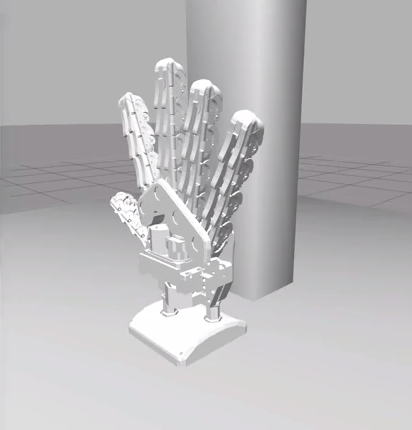
\includegraphics[width=0.45\textwidth]{open.png}
\hspace{1pt}
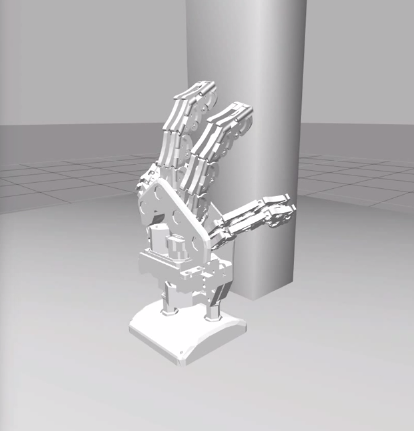
\includegraphics[width=0.45\textwidth]{close.png}
\caption{The Pisa/IIT SoftHand simulated in Gazebo at full open (left) and close (right) commanded configurations.}
\label{fig:soft_hand_gazebo}
\end{figure}

\subsubsection{Joint state estimation}

At this point, there are two on going works regarding this issue that we expect to converge in a sensor fusion approach during the time remaining on the project. The first one is presented in DR 3.1, where an IMU-based glove provides an accurate estimate of the joint angles. The second approach is a simulator-in-the-loop extended Kalman filter, where the simulation play the role of the system model to give the estimated joint values, and motor position (via a position encoder) and effort (estimated from the current measurement) are used as measurements to update the filter via the adaptive synergy transmission equations implemented in the transmission interface as described above. This work is being submitted to IROS 2015, for more details see the attached at~\href{}{this link}.
\subsection{Software: KIT Head package}
\label{sec:kithead}

The Karlsruhe humanoid head~\cite{Asfour2008KITHead} was acquired as the testbed for active gaze strategies. Fig.~\ref{fig:kit_head} shows a picture of the real device.

\begin{figure}
\centering
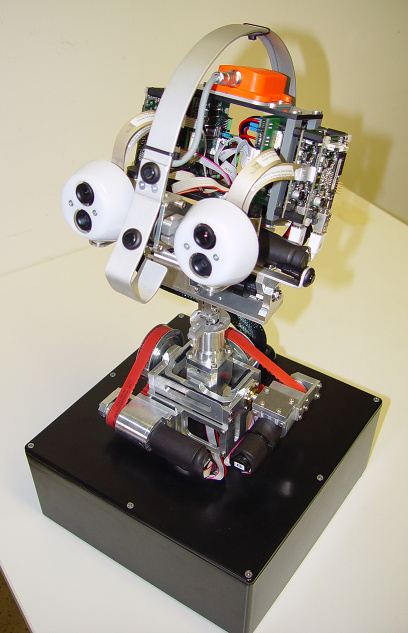
\includegraphics[width=0.25\textwidth]{kithead.png}
\caption{The Karlsruhe humanoid head.}
\label{fig:kit_head}
\end{figure}

\subsubsection{Hardware interface}

The real hardware interface is still to be developed. The simulated hardware interface considers the default behavior of a robot using position controlled motors. This is good enough for the planning and simulation environment, specially to test active gaze control. In order to do that, we added the simulation of point cloud acquisition, as well as two RGB cameras per eye to be as close as possible to what the Humanoid Head offers. The simulation of the cameras is described next.

\subsubsection{Camera simulation}
There are out-of-the-box camera plug-ins for both kind of cameras, RGB and RGB-D. Both are used in the simulated head. The point cloud and images are published in an uncalibrated frame as well as in the real robot could be. Real calibration values can be loaded to have camera and robot  under the same tree of connectivity. Parameters such as noise and noise type can be set to test active gaze control and object recognition in ideal and not so ideal conditions. Fig.~\ref{fig:head_vision} shows the simulated RGB and RGB-D cameras mounted on the eyes and forehead. Note that, the robot model has been set to almost transparent in the visualizer at the bottom, and the point cloud is overlayed covering the hand and wrist.

\begin{figure}[h!]
\centering
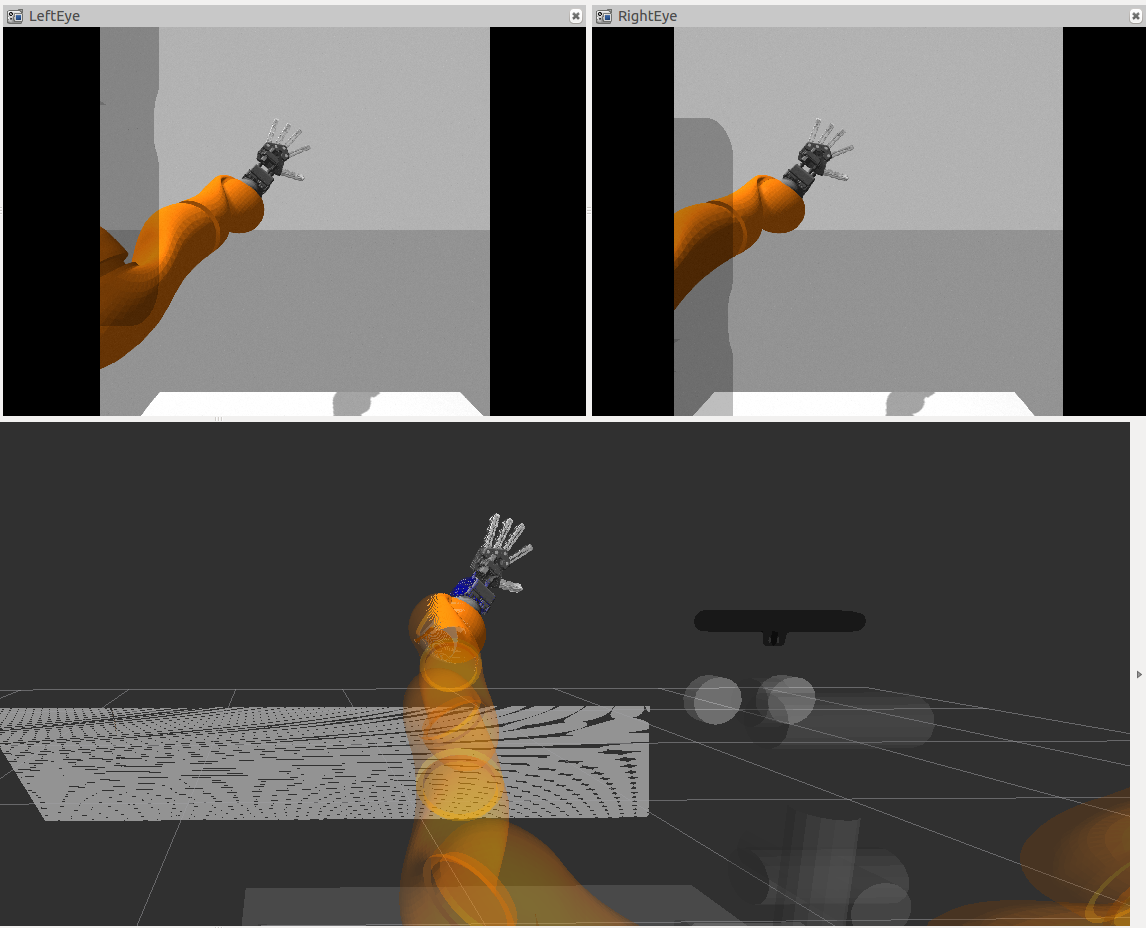
\includegraphics[width=0.7\textwidth]{headVision.png}
\caption{Simulation of RGB (top) and RGB-D (bottom) cameras available in the real humanoid head.}
\label{fig:kit_vision}
\end{figure}
% \section{Conclusions and Future Works}
% The present work had the aim of implementing an extended set of different classes of controllers for the robotic arm KUKA LWR IV, exploiting a flexible system which is rapidly growing in the field of robotics, including research and whole industrial processes. In fact, all the code produced could not only be accessed and used from users operating the same robot, but ideally from everyone who works with ROS, at least performing some minor edits to fit their needs. Thinking about future works starting from this project, it could be interesting the extension to a bimanual system in a human-like arms configuration. For example, taking advantage of the Stack of Tasks framework could be also provided obstacle and collision avoidance, making easier the interaction between the robot and humans or the handling of more complex operations. 
% \newpage

\bibliographystyle{IEEEtran}
\bibliography{../shared_bibliography/abbreviations,bibliography/MS42}

\end{document}
